\documentclass%[handout]
{beamer}

\mode<presentation>
{
  \usetheme{Warsaw}
  %\setbeamercovered{transparent}
}

\usepackage[english]{babel}
\usepackage[latin1]{inputenc}
\usepackage{times}
\usepackage[T1]{fontenc}


\title[Mid-term Project Evaluation]
{Activity Recognition using Text Mining and Object Recognition}

\author[Niranjan A. Viladkar]
{\fontsize{8pt}{1em} \selectfont Niranjan A. Viladkar \\Under the guidance from \\ Dr. Subhashis Banerjee and Dr. Parag Singla}

\institute
{
	Department of Computer Science\\
	IIT Delhi
}
\date{\fontsize{8pt}{1em} \selectfont May 13, 2013}


%\titlegraphic{
\includegraphics[height=2cm]{iitlogo-21.jpg}}

% Delete this, if you do not want the table of contents to pop up at
% the beginning of each subsection:
%\AtBeginSubsection[]
%{
%  \begin{frame}<beamer>{Outline}
%    \tableofcontents[currentsection,currentsubsection]
%  \end{frame}
%}


% If you wish to uncover everything in a step-wise fashion, uncomment
% the following command: 

\beamerdefaultoverlayspecification{<+->}


\begin{document}

\begin{frame}
  \titlepage
\end{frame}


\begin{frame}{Table of Contents}
  \tableofcontents%[pausesections]
\end{frame}

 \section{Problem Statement}

\subsection{Activity Recognition}

\begin{frame}{What is Video Activity Recognition?}
	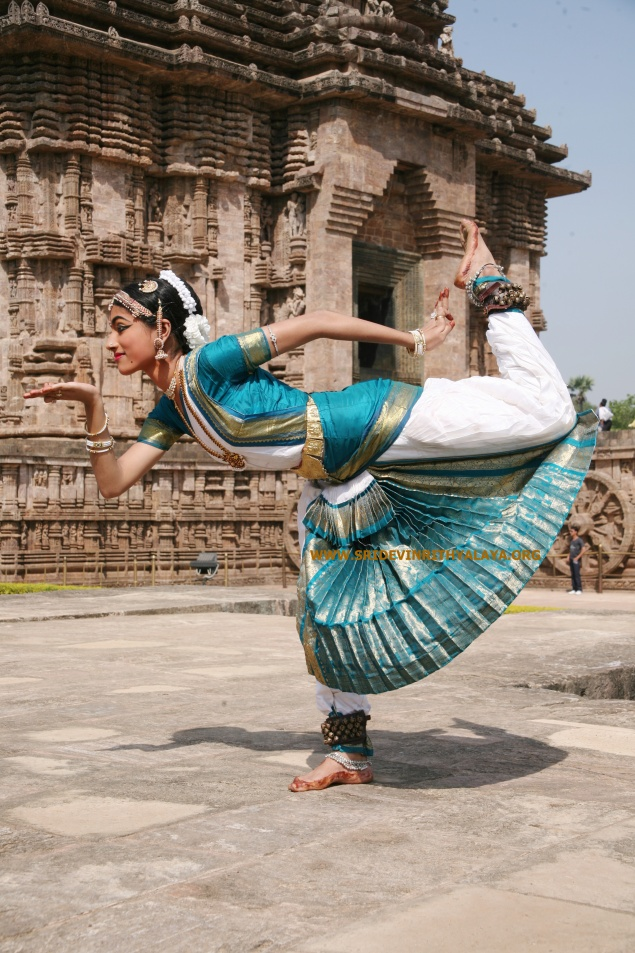
\includegraphics[scale=0.2]{Dancing01.jpg}
\end{frame}


\begin{frame}{Learning Realistic Human Actions from Movies}{Ivan Laptev et al.}
	\begin{enumerate}
		\item Previous Attempts in Simplified Settings
		\item Supervised Learning
		\item Possible to Work with Long Videos / Movies
	\end{enumerate}
\end{frame}



\subsection{Object Detection and Text Mining}

\begin{frame}{Improving Video Activity Recognition}{ Using Object Recognition and Text Mining. Tanvi S. Motwani and Raymond J. Mooney}
	\begin{itemize}
		\pause
		\item Text Mining to Determine Classes
			\begin{itemize}
				\item Get Verbs - Part of Speech Tagger
				\item Stem the Verbs
				\item Cluster Similar Verbs using WordNet 
				\item These Clusters form Classes
			\end{itemize}

		\item Initial Probability Distribution
			\begin{itemize}
				\item From STIPs, HoG and HoF, form Vocabulary
				\item Train a Standard Video based Activity Classifier
			\end{itemize}
	\end{itemize}
\end{frame}

\begin{frame}{Improving Video Activity Recognition}{ Using Object Recognition and Text Mining. Tanvi S. Motwani and Raymond J. Mooney}
	So, till now, we have
	\begin{itemize}
		\pause
		\item Determined Classes
		\item Got Initial Probability Distribution
	\end{itemize}
	\pause

  
	\vskip0pt plus.5fill
	Now,
	\begin{itemize}
		\item Detect Objects
		\item Correlations between Activities and Objects 
			\begin{itemize} 
				\pause \item From raw text, get occurrences and co-ocurrences count
			\end{itemize}
		\item Find $P( Activity | Object )$ thus find $P( Activity | Features )$
		\item Initial Probabilities vs Combined Probabities
	\end{itemize}
\end{frame}
\subsection{Unsupervised Activity Detection}
\begin{frame}{Latent Topic Model-Based Group Activity Discovery}{T.A. Faruquie, S. Banerjee, P. Kalra}
	\begin{itemize}
		\item Form Vocabulary
		\item Find Distribution of an Activity over Clips
		\item Activities having Similar Distributions are Group Activities
	\end{itemize}
\end{frame}

\section{Direction of Project}
\subsection{This Semester Work}
\begin{frame}{Idea of This Semester Work}
	\pause
	The Best way to have a good idea is to have many ideas. \\
	\hspace{1 cm}- \textbf {Linus Pauling}

	\pause
	\begin{enumerate}
		\item Object Detection using Scene Information
		\item Use Text to Detect Objects
		\item Improve Object Detector Using Feedback
	\end{enumerate}

\end{frame}


% All of the following is optional and typically not needed. 
\appendix
\section<presentation>*{\appendixname}
%\subsection<presentation>*{References}

\begin{frame}[allowframebreaks]
  %\frametitle<presentation>
  {References}
    
  %\begin{thebibliography}{0}
    
%  \beamertemplatebookbibitems
  % Start with overview books.

 % \bibitem{Author1990}
 %   A.~Author.
 %   \newblock {\em Handbook of Everything}.
 %   \newblock Some Press, 1990.
 
    
  %\beamertemplatearticlebibitems
  % Followed by interesting articles. Keep the list short. 

  %\bibitem{Laptev2008}
    Learning Realistic Human Actions From Movies
    \\Ivan Laptev, Marcin Marszalek, Cordelia Schmid, Benjamin Rozenfeld
    {\em Proc. CVPR, 2008}.

	\vskip15pt 
    
    %\bibitem{Motwani2012}
	Improving Video Activity Recognition Using Object Recognition and Text Mining
	\\ Tanvi S. Motwani and Raymond J. Mooney
	{\em Proc. ECAI-2012}.

	\vskip15pt

    %\bibitem{Tanveer2011}
	    Latent Topic Model-based Group Activity Discovery
	\\ T.A. Faruquie, S. Banerjee, P. Kalra
	{\em Vis Comput (2011) 27:1071-1082}.


  %\end{thebibliography}
\end{frame}

\end{document}


